\documentclass{beamer}


% PACKAGES==========================================================================================
\usepackage{hyperref}
\usetheme[hideothersubsections]{PaloAlto}
\useinnertheme{rectangles}
\usecolortheme{beaver}
\usepackage[version=3]{mhchem}
\usepackage{caption}
\usepackage{textpos}
\usepackage{amsmath}
\usepackage{etoolbox}
\usepackage{wrapfig}
\usepackage{multicol}
\usepackage[caption=false]{subfig}
%\usepackage[font=small,skip=0pt]{caption}



% SETTINGS==========================================================================================
\setbeamerfont{caption}{series=\normalfont,size=\fontsize{5}{5}}
\setbeamercolor{section in sidebar}{fg=black}
\setbeamercolor{section in sidebar shaded}{fg=lightgray}%section in sidebar.fg!40!bg}
%\setbeamercolor{section in sidebar}{fg=black}            %color of the active section
%\setbeamercolor{section in sidebar shaded}{fg=gray}     %color of the inactive section
\setbeamercolor{subsection in sidebar}{fg=darkred}         %color of the active subsection
\setbeamercolor{subsection in sidebar shaded}{fg=darkgray}  %color of the inactive subsection
\setbeamercolor{title in sidebar}{fg=black}              %color of the presentation title
%\setbeamercolor{author in sidebar}{fg=...}             %color of the author  
%\setbeamertemplate{section in toc shaded}[default][10]
 
 
\makeatletter
\patchcmd{\insertverticalnavigation}%
{\ifx\beamer@nav@css\beamer@hidetext{\usebeamertemplate{section in sidebar}}\else{\usebeamertemplate{section in sidebar shaded}}\fi}%
{{\usebeamertemplate{section in sidebar}}}{}{}
\makeatother 
 
 
\setbeamerfont{block body}{size=\tiny}
%\setbeamertemplate{blocks}[square][shadow=false]
\setbeamertemplate{blocks}[default]
\setbeamertemplate{bibliography item}[text]
\setlength{\parindent}{0pt}
\setbeamertemplate{caption}[numbered]


\defbeamertemplate*{section in toc}{my theme}
{\leavevmode\leftskip=0.5em\large{\usebeamercolor[fg=darkred]{titlelike}\inserttocsectionnumber.} \inserttocsection\par}

\defbeamertemplate*{subsection in toc}{my theme}
{\leavevmode\leftskip=0.5em\normalsize{\usebeamercolor[fg=darkgray]{titlelike}\inserttocsectionnumber.\inserttocsubsectionnumber.} \inserttocsubsection\par}



% Define footer
\setbeamertemplate{footline}{bg=primary}
\makeatother
\setbeamertemplate{footline}
{
    \leavevmode%
    \hbox{%
    \begin{beamercolorbox}[wd=.4\paperwidth,ht=2.25ex,dp=1ex,center]{author in head/foot}%
       \usebeamerfont{author in head/foot}\insertshortauthor\ (Chris Ngigi - DEC I)
    \end{beamercolorbox}%
    
    \begin{beamercolorbox}[wd=.4\paperwidth,ht=2.25ex,dp=1ex,center]{title in head/foot}%
        \usebeamerfont{title in head/foot}\insertshorttitle
        \hfill
    \end{beamercolorbox}    
        
    \begin{beamercolorbox}[wd=.2\paperwidth,ht=2.25ex,dp=1ex,center]{title in head/foot}%
        \usebeamerfont{title in head/foot}
        \hfill    
        \hspace{2em}\insertframenumber/\inserttotalframenumber
    \end{beamercolorbox}}%
}

\beamertemplatenavigationsymbolsempty  % disable navigation
\setbeamertemplate{sidebar}{%
   \vspace*{0cm}
    \vspace*{\fill}
   \vspace*{0.1cm}
   \setbeamersize{sidebar width left=2cm}
   
\includegraphics[width=0.55cm]{./figs/utias_logo_blue.jpg}
}
    
\setbeamerfont{section number projected}{family=\rmfamily,series=\bfseries}
\setbeamercolor{section number projected}{bg=lightgray,fg=darkred}
\setbeamertemplate{sections/subsections in toc}[square]

\addtobeamertemplate{frametitle}{}{%
\begin{textblock*}{1cm}(-1.8cm,-1.2cm)

\includegraphics[height=1cm,width=1cm]{./figs/utias-logo2.jpg}
\end{textblock*}}

\makeatletter
\patchcmd{\beamer@sectionintoc}{\vskip1.5em}{\vskip0.5em}{}{}
\patchcmd\insertverticalnavigation{\dohead}{\vskip-35pt\dohead}{}{}
\makeatother


% ==================================================================
% NOW MAIN DOCUMENT

%%========================================================================

\title[]{Development of h-p Adjoint-based error estimation for LES of reactive flows }
\author[]{{Christopher Ngigi \texorpdfstring{\\ \tiny{Ph.D. Pre-Candidate} \\} \footnotesize Supervisor: Prof. C. P. T. Groth}}
\titlegraphic{
\includegraphics[width=0.15\textheight]{./figs/utias_logo_blue.jpg}}
\institute[]{Doctoral Examination Committee \\ Meeting I \\ University of Toronto, Institute for Aerospace Studies}
\date[]{April 6, 2015}
	
%%========================================================================

\begin{document}

\addtocounter{framenumber}{-1}
\begingroup
\makeatletter
\setlength{\hoffset}{-.5\beamer@sidebarwidth}
\makeatother
\begin{frame}[plain]
    \titlepage	
\end{frame}

%==========================================================================================
\begin{frame}[plain,c]
\centering
\begin{minipage}[t][1\textheight]{1\textwidth}
\begin{alertblock}{\large{Outline: }}
\small

\tableofcontents[hideallsubsections]

\end{alertblock}
\end{minipage}
\end{frame}
\endgroup

%===========================================================================================

% this section adds a mini TOC between sections. CTRL+U to activate
%\AtBeginSection[]
%{
%     \begin{frame}[plain,c]
%     \begin{minipage}[t][1\textheight]{0.8\textwidth}
%     %\setbeamercolor{section in toc shaded}{use=structure,fg=lightgray}
%     \setbeamercolor{section in toc}{fg=darkred}
%     \setbeamercolor{subsection in toc}{fg=darkgray}
%          
%     %
\includegraphics[width=1.5cm]{./figs/utias_logo_blue.jpg}
%     \begin{alertblock}{\large{Section:}}
%     \tiny
%     \tableofcontents[currentsection, sectionstyle=show/shaded, subsectionstyle=show/show/hide]
%     \end{alertblock}
%     \end{minipage}
%     \end{frame}
%}

%==========================================================================

\section{Introduction}
\subsection{Computing power}
\begin{frame}%[allowframebreaks]
\frametitle{Introduction}
\vspace{-6pt}
\scriptsize 
Cost of experiment vs numerical simulation
\begin{itemize}
\tiny
\item Computational Fluid Dynamics (CFD) developed to reduce the time and cost of prototypes in fluid flow experiments. 
\item Complexities may be expensive to set up in experimental modeling
\item CFD methods and models have been developed to capture this phenomenon to varying extents of accuracy
\end{itemize}
Moore's law: Computing power $\approx$ doubles every 2 years
\vspace{-1mm}
\begin{figure}[h!]
%\centering
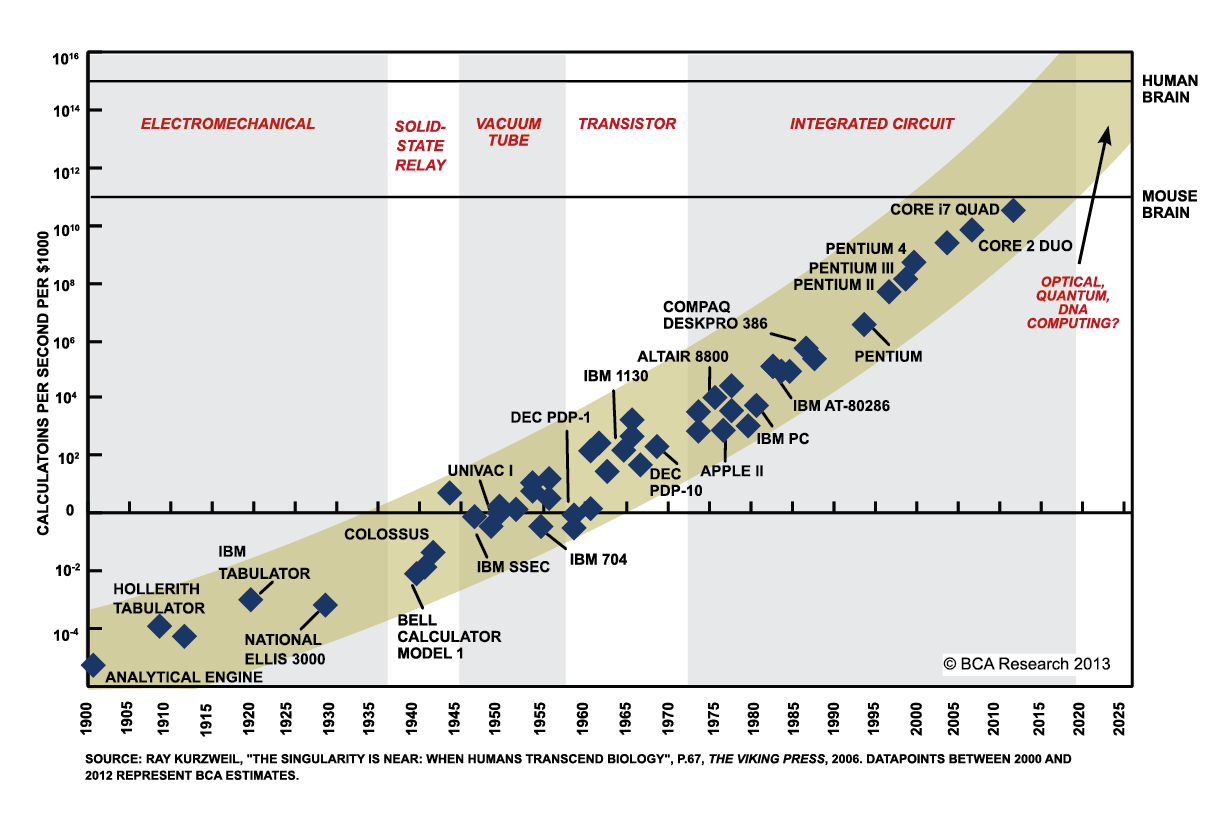
\includegraphics[height=0.47\textwidth, trim=0cm 1.2cm 0 1.2cm,clip=true]{./figs/MooresLaw.png}
\caption{Moore's Law over the years [BCA Blog] \cite{MooreLaw}]}
\label{fig:Moore}
\end{figure}
\end{frame}

%==========================================================================

\subsection[experimental]{Turbulent combustion - experimental}
\begin{frame}%[allowframebreaks]
\frametitle{Turbulent combustion - experimental}
\small{Turbulent combustion: real fluid flows almost always involve turbulence. Large eddy simulation (LES) - technique to achieve higher accuracy than Reynolds' averaged Navier Stokes (RANS) at lower computational cost (time, resources) than direct numerical simulation (DNS).}
\begin{minipage}[0.5\textheight]{\textwidth}
\begin{columns}[T]
\begin{column}{0.65\textwidth}
\vspace{20pt}
\small{Lifted turbulent Ethylene ($C_2H_4$) jet flame issuing into a concentric co-flow of air. Zone between flame-base and nozzle may have partial premixing. Fuel and air temperature, pressure near standard [K{\"o}hler 2006] \cite{Kohler}}
\begin{itemize}%[<+->]
\tiny
\setlength\itemsep{-0.7mm}
\item Dimensions: Nozzle diameter = 2.0 mm; Co-flow air annulus diameter = 140 mm\\
\item Exit Reynolds number: 10000
\item Air mass flow: 320 g/min 
\item Mean fuel jet velocity: 44 m/s 
\end{itemize}
\end{column}

\begin{column}{0.3\textwidth}
\vspace{0pt}
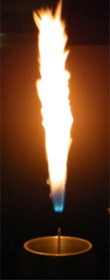
\includegraphics[height=1.4\textwidth]{./figs/dlrflame.png}
\newline
\tiny
[K{\"o}hler 2006] \cite{AdelaideISF}
\end{column}
\end{columns}
\end{minipage}
\end{frame}

%==========================================================================

\subsection[simulation]{Turbulent combustion - simulation}
\begin{frame}%[allowframebreaks]
\frametitle{Turbulent combustion - simulation example}
\scriptsize
{Considering that DNS resolves all the scales, LES models sub-filter scales (SFS) while resolving the larger scales, and that RANS models all the scales, then we can expect the most accurate to be DNS, then LES, then RANS. Computational results that Yang, Pope and Chen  obtained are:}
\vspace{-25pt}
\begin{figure}
\label{fig:DNSLES}
\centering
\subfloat[\tiny{temperature in x-y plane: DNS (l), LES/PDF (r)} \label{fig:contourDNS}]{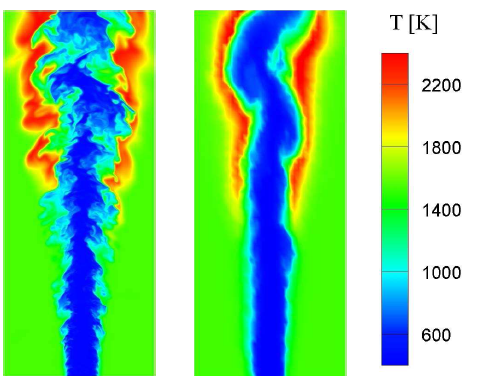
\includegraphics[width=0.7\textheight]{./figs/Temperatures.png}}
\subfloat[\tiny{Mean temperature :DNS and LES} \label{fig:meanTemp}]
{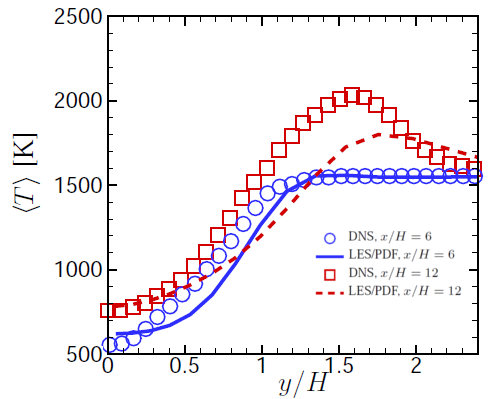
\includegraphics[width=0.65\textheight]{./figs/Temp_DNS_LES2.png}}
\tiny{\caption{\tiny{DNS and LES results for a turbulent Ethylene jet flame in hot co-flow, [Yang et al, 2013 \cite{Pope}]}}}
\end{figure}
\end{frame}

\begin{frame}%[allowframebreaks]
\frametitle{Turbulent combustion - simulation example cont'd}
\scriptsize
Their numerical setup:
\begin{itemize}
\item DNS 
\begin{itemize}
\tiny
\item Grid points $ = 1.3 \times 10^9$.  
\item Computational cost $ = \approx 14 \times 10^6$ CPU hours.
\item Computational domain $ = 3D $ cuboid  $L_x \times L_y \times L_z = 15H \times 20H \times 3H$ in the streamwise x-, transverse y-, and spanwise z-directions, where H = 2 mm is the jet width. Boundary conditions (BCs) are inflow/outflow in x and y, while periodic in z.
\end{itemize}
\item LES
\begin{itemize}
\tiny
\item Grid points $ \approx 8.3 \times 10^3$.  
\item Computational cost $ = $ not specified - expected to be several orders of magnitude \textit{lower}.
\item Computational domain $ = 3D $ cuboid $  L_x \times L_y \times L_z = 15H \times 30H \times 3H$. (larger y to move the transverse boundary away from the central turbulent jet, which can avoid the artifact of the Dirichlet boundary condition on entrainment near the jet.)
\end{itemize}
\end{itemize}
The results they obtained for mean temperature reveal good agreement between LES and DNS at x/H = 6, with lower-than-predicted values at x/H = 12. They anticipate mean temperature prediction to improve with finer mesh resolution in the LES grid.

\end{frame}
%=========================================================================

\section[Scope]{Scope of research}
\begin{frame}%[allowframebreaks]
\frametitle{Scope of research}
\scriptsize
\begin{itemize}
\item Reducing numerical error
\item High Order ... CENO
\item Explicit filtering
\item Adjoint based error estimation
\item Using h and p adapatation
\end{itemize}
\end{frame}

\subsection{this will be a subsection}

\subsection{this will be another subsection}

\subsection{this will be the last subsection}

%==========================================================================

\section[Methodology]{Methodology}
\begin{frame}%[allowframebreaks]
\frametitle{Methodology}
\scriptsize
\begin{itemize}
\item Favre Averaged Governing Equations
\item Large Eddy Simulation:
  \begin{itemize}
  \scriptsize
   \item Explicit Filtering
   \item Some LES errors: Aliasing, Commutation
   \item Sub-filter scale (SFS) modeling
  \end{itemize}
\item High-order finite volume methods: CENO technique - benefits of higher accuracy on a coarse mesh
\item AMR
   \begin{itemize}
   \scriptsize
   \item Block-based AMR: speed and parallelization
   \item Anisotropic vs Isotropic: how cell count (computational cost) can be reduced
   \item Now the non-uniform vs the uniform block modification
   \item Mesh geometry: CFFC can deal with cartesian or curvilinear coordinates - is this via using mapping functions for reference elements?
   \end{itemize}
\end{itemize}
\end{frame}

%==========================================================================
\section[Framework]{Existing framework}
\begin{frame}%[allowframebreaks]
\scriptsize
\frametitle{Existing framework}
\begin{itemize}
\item The CFFC code already includes the following required features:
\item Block-Based : people, year
\item AMR:
\item Deconick's research on explicit filters
\item High Order FVM with CENO:
\item Scott's work/input: Newton iterations and GMRES solver
\item Lucie's non-uniform approach - improves accuracy of flux evaluations and reduces computational cost for anisotropic
\item PCM-FPI combustion modelling: modeled by F. Hernandez-Perez 
\item Initial adjoint analysis done by Martin for the advection equations
\end{itemize}
\end{frame}

%==========================================================================


\section[Error]{Overview of error}
\begin{frame}%[allowframebreaks]
\frametitle{Overview of error}
\vspace{-5pt}
\begin{minipage}[t][0.7\textheight]{1\textwidth}
\scriptsize
\vspace{-20pt}
\begin{block}{Likely sources of error}
\vspace{-10pt}
\begin{figure}[h!]
%\centering
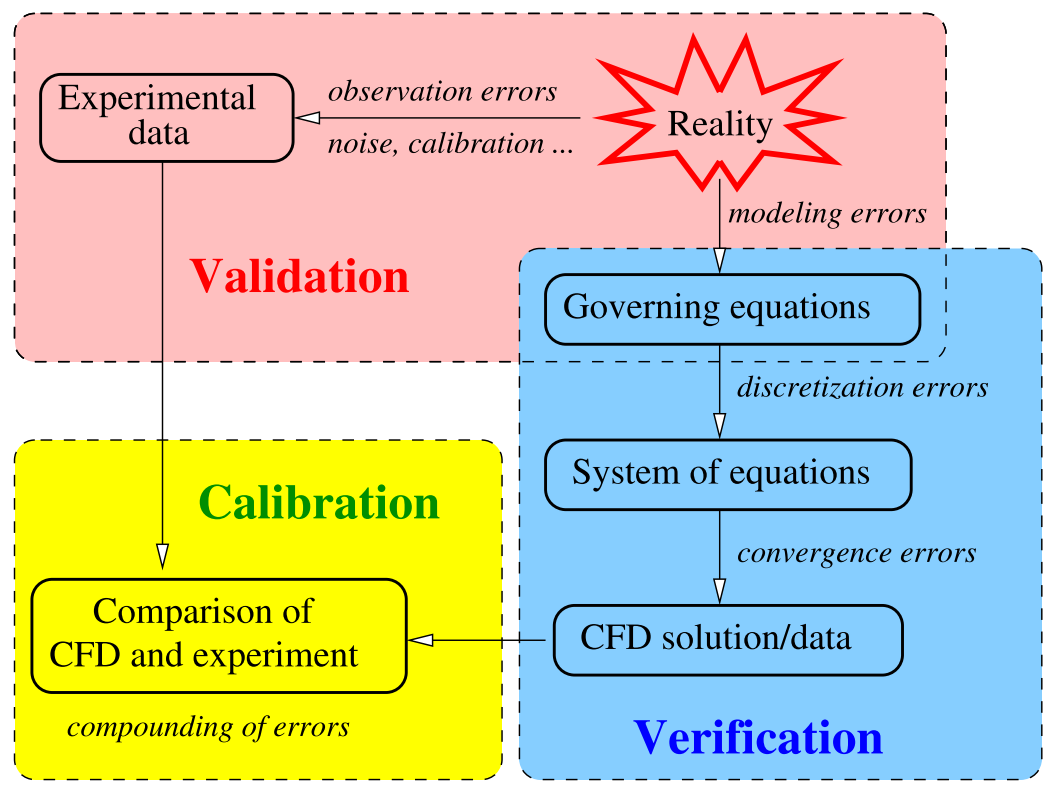
\includegraphics[height=0.47\textwidth]{./figs/Error.png}
\vspace{-5pt}
\caption{Some sources of error [Fidkowski 2012]}
\label{fig:Fidk}
\end{figure}
\vspace{-20pt}
\end{block}
\end{minipage}
\vspace{-8pt}
\tiny
Modelling error chiefly arises from
\begin{itemize}
\item LES: Aliasing error, commutation error
\item Mesh: selection of the mesh refinement, types of cells, configuration to bulk flow direction
\end{itemize}
Discretization error chiefly arises from
\begin{itemize}
\item Truncation error - how high order reduces this
\item Solution error
\end{itemize}
\end{frame}


%==========================================================================

\section[AMR]{Adaptive mesh refinement}
\begin{frame}%[allowframebreaks]
\frametitle{Adaptive mesh refinement (AMR)}
\scriptsize
\begin{itemize}
\item Benefits of AMR
\item How the block-based technique works
\item Ghost cells for intercommunication
\item Current stencils
\item how the high-order will affect the current stencil
\item use radial sphere diags
\end{itemize}
\end{frame}





%==========================================================================

\section[FVM]{High order FVM, CENO and LES}
\subsection{High order FVM}
\begin{frame}%[allowframebreaks]
\frametitle{High order finite volume method}
\scriptsize
An explanation on h.o FVM.
how the high-order works, and how it reduces numerical error.
separate slide of other groups researching this: Ihme and Poinssot. show some of their results
\end{frame}


\subsection{CENO}
\begin{frame}
\scriptsize
\frametitle{Central essentially non-oscillatory (CENO) scheme}
\begin{itemize}
\item Lucien's work
\item Ramy's work
\item Marc Charest's work
\item Luiz's work
\end{itemize}
\end{frame}

\subsection{LES}
\begin{frame}
\frametitle{Large Eddy Simulation}
\scriptsize

Give an overview

Explicit filtering. [Deconinck, 2008]
\begin{itemize}
\item one point about explicit vs implicit filtering
\item another point about the filtering
\end{itemize}
\end{frame}


%===== ADJOINT =====================================================================
\section[Error estimates]{Error estimation}

\subsection{Foundation}
\begin{frame}
\frametitle{Foundation for error estimation}
\scriptsize
Basis for selective mesh refinement - we would like to refine the mesh where the cells have a very critical effect on the solution, while coarsening the less critical areas to save on computational cost.\newline 
Basically, there are two types of error estimation procedures available:
\begin{itemize}
\item a priori error estimators:  these predict the long-term behavior of the errors in the discretization. They are not actually designed to approximate the error estimate for a given mesh. 
\item a posteriori error estimators: these use the simulation results to derive estimates of solution errors. Furthermore, these results are used to guide adaptive schemes:
\begin{itemize}
\scriptsize
\item where either the mesh is locally refined (h-version) 
\item where the polynomial degree is raised (p-method)
\end{itemize}
\end{itemize}
Two main a posteriori approaches are the:
\begin{itemize}
\item gradient-based : [Bibb et al, 2006] [Giles and Pierce, 2000]
\item adjoint-based : [Giles and Pierce, 2000][Venditti and Darmofal - 2000,2002][Fidkowski and Darmofal, 2011] 
\end{itemize}
\end{frame}


\subsection[Gradient]{A background on gradient/physics-based refinement}
\begin{frame}%[allowframebreaks]
\scriptsize
\frametitle{A background on gradient/physics-based refinement}
In these simulations, the mesh or discretization order is changed based on the rates of change of (physical) solution variables.\newline
Where the change occurs most rapidly over a few mesh cells, then over this location the mesh resolution can be increased (higher mesh refinement), or the scheme order can be increased, effectively using a higher order discretization over these cells.

\begin{itemize}
\item The reasoning behind this is to have enough cells to capture the changes as \textit{smoothly} as possible.
\item Once refinement is completed, the solution is re-run and the gradients re-evaluated. Changes made as necessary. Error can be compared to a higher discretization (h or p) solution.
\item This is the present utility in the anisotropic and isotropic AMR functionality of the CFFC code used by the CFD and Propulsion group.
\item main disadvantages of the gradient based approach [Giles and Pierce, 2000]:
\begin{itemize}
\tiny
\item for each separate state variable, a separate simulation must be run to evaluate the desired mesh resolution - increases computational time
\item gradient-based approach can only deal with continuous functionals as opposed to discrete optimization functionals
\item inability to deal with functions that have multiple minima. In this latter case, the gradient-based technique will generally converge to the nearest local minima, whose value may not represent overall system minimum.
\end{itemize}
\end{itemize}
\end{frame}



\subsection[Adjoint]{About the adjoint}
\begin{frame}%[allowframebreaks]
\scriptsize
\frametitle{About the adjoint}
To make error estimation more relevant to engineering applications: assess the error made in predicting an integral quantity which represents an engineering output. This output is the functional. For example,the output can be the average pressure on a wall. The adjoint technique is a sensitivity analysis, that measures the rates of change of a design functional to a given change in the residual.\newline
The adjoint has two main formulations [Venditti and Darmofal, 2000]:
\begin{itemize}
\item continuous:
\begin{itemize} 
\tiny
\item An objective function is formed to enforce the flow conditions (i.e. primal nonlinear PDEs). 
\item Consider linear perturbations to the primal flow variables: the objective function should remain constant w.r.t the perturbations.
\item Hence obtain analytical adjoint equations. Obtain appropriate boundary conditions, and discretized directly. Primary benefit - offers insight into the nature of the adjoint solution.
\end{itemize}
\item discrete 
\begin{itemize}
\tiny
\item begin with the nonlinear discrete residual equations from the primal problem
\item apply linear perturbations to these. 
\item If adjoint consistent (discrete adjoint = continuous adjoint), no need for B.C. specification -automatically incorporated via the primal residual.   
\item thus obtain a linear system of equations - only need linear sensitivities of the functional and the Jacobian matrix associated with the primal residual.
\end{itemize}
\end{itemize}
\end{frame}

\begin{frame}
\frametitle{Discrete adjoint}
\scriptsize
For these initial stages, beginning with the discrete formulation of the adjoint
\begin{minipage}[t][0.6\textheight]{0.75\textwidth}
\scriptsize
\vspace{-10pt}
\begin{exampleblock}{Discrete Adjoint}
\[
\left( \frac{\partial{R}}{\partial{U}} \right)^T ~\Psi~ = -\left( \frac{\partial{J}}{\partial{U}} \right)^T
\]
\text{yielding a linear system of equations:}
\[
Ax = b
\]
\tiny
Where:
\begin{itemize}
\item \textbf{$J$} = the functional
\item \textbf{$R$} =  the residual
\item \textbf{$\psi$} = the adjoint vector
\end{itemize}
\end{exampleblock}
\end{minipage}

Methods to evaluate $\frac{\partial{J}}{\partial{R}} $  for the discrete adjoint:
\begin{itemize}
\scriptsize
\item Finite differencing {\color{red}[citations]}
\item Forward linearization with automated differentiation {\color{red}[citations]}
\item Adjoint method {\color{red}[citations]}
\item Complex step {\color{red}[citations]}
\end{itemize}


\end{frame}


%=====================================================================

\subsection[Usage]{Basis of refinement: h and p}
\begin{frame}%[allowframebreaks]
\frametitle{\scriptsize{Usage of the adjoint as a basis of refinement: h and p}}
\scriptsize
Some of the groups using \textbf{adjoint with AMR}
\begin{itemize}
\item Becker and Rannacher [2001] - An Optimal Control Approach to a Posteriori Error Estimation in Finite Element Methods
\item Fidkowski and Darmofal [2011] - Review of Output-Based Error Estimation and Mesh Adaptation in Computational Fluid Dynamics
\item Hartmann [2006] - Error Estimation and Adjoint-based Adaptation in Aerodynamics
\item Nemec and Aftosmis [2007] - Adjoint Error Estimation and Adaptive Refinement for Embedded-Boundary Cartesian Meshes
\item Nemec, Aftosmis, and Wintzer [2008] - Adjoint-Based Adaptive Mesh Refinement for Complex Geometries
\item Hartmann, Held and Leicht [2010] - Adjoint-based error estimation and adaptive mesh refinement for the RANS and k-ω turbulence model equations
\item Woopen, May and Sch{\"u}tz [2013] - Adjoint-Based Error Estimation and Mesh Adaptation for Hybridized Discontinuous Galerkin Methods
\item Li, Allaneau and Jameson [2011] - Continuous Adjoint Approach for Adaptive Mesh Refinement
\item Diskin and Yamaleev [2011] - Grid Adaptation Using Adjoint-Based Error Minimization
\end{itemize}
\end{frame}

%-----------------------------------------------------------------

\subsection[Estimation]{Error estimation indicators}
\begin{frame}
\scriptsize
\frametitle{Error estimation indicators}
All about residual weighting (flag for refinement) and a 1D cartoon example, perhaps, of restriction/prolongation
\begin{itemize}
\item projecting onto fine space
\item restricting onto coarse space
\item getting the error in the residual and using this as a flag for refinement
\end{itemize}
\end{frame}

%-----------------------------------------------------------------

\subsection{Steady vs unsteady}
\begin{frame}
\scriptsize
\frametitle{Steady vs unsteady}
Lastly: treatment of steady vs unsteady adjoints
\end{frame}

%-----------------------------------------------------------------

\subsection{Benefits}
\begin{frame}
\scriptsize
\frametitle{Benefits of the adjoint approach}
Expected benefits of adjoint vs gradient based methods
\end{frame}

%-----------------------------------------------------------------

\subsection{Mesh adaptation}
\begin{frame}
\scriptsize
\frametitle{Mesh adaptation based on adjoint}
This is a separate slide on mesh adaptation as based on the adjoint. Enough diagrams from venditti and darmofal, fidkowski
\end{frame}

%==========================================================================


%==========================================================================
\section[Usage]{Usage}

\begin{frame}%[allowframebreaks]
\frametitle{How we can use this}
\scriptsize
\begin{itemize}
\item using it for mesh refinement - how some previous groups used this
\item how we can link mesh adaptation AMR to the adjoint via h
\item how we can use p based refinement
\end{itemize}
\end{frame}


%==========================================================================
\section[Progress]{Progress to date}

\begin{frame}[shrink=20]%[allowframebreaks]
\frametitle{Poisson problem}
\scriptsize
\begin{minipage}[t][1\textheight]{1\textwidth}
\vspace{-20pt}
\begin{exampleblock}{Creating and solving linear systems in parallel implementation - trilinos and MPI}
\vspace{-20pt}
\begin{figure}
\label{fig:Poisson}
\centering
\subfloat[\tiny{2D case on $N^2 = 200^2$} \label{fig:Poiss2D}]{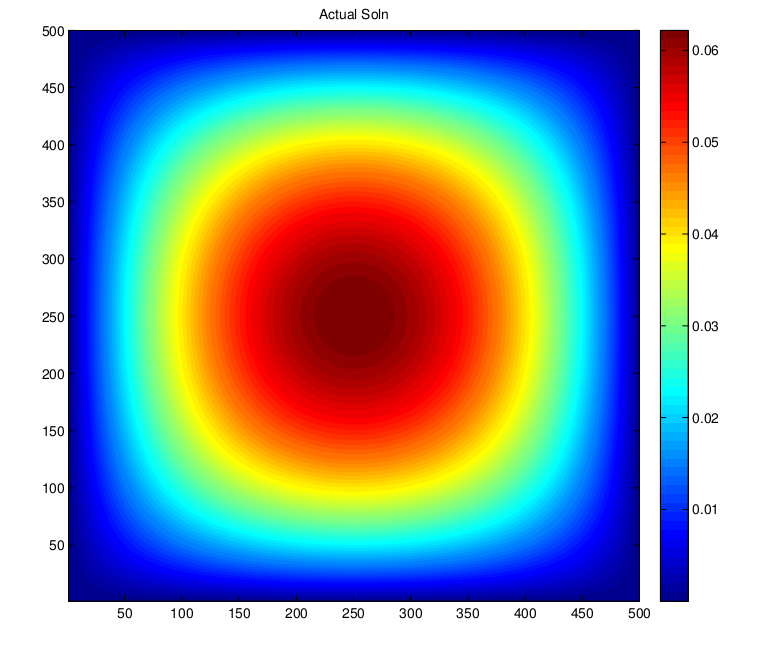
\includegraphics[width=0.7\textheight]{./figs/Poisson2D.png}}
\subfloat[\tiny{3D case on $N^3 = 100^3$} \label{fig:Poiss3D}]{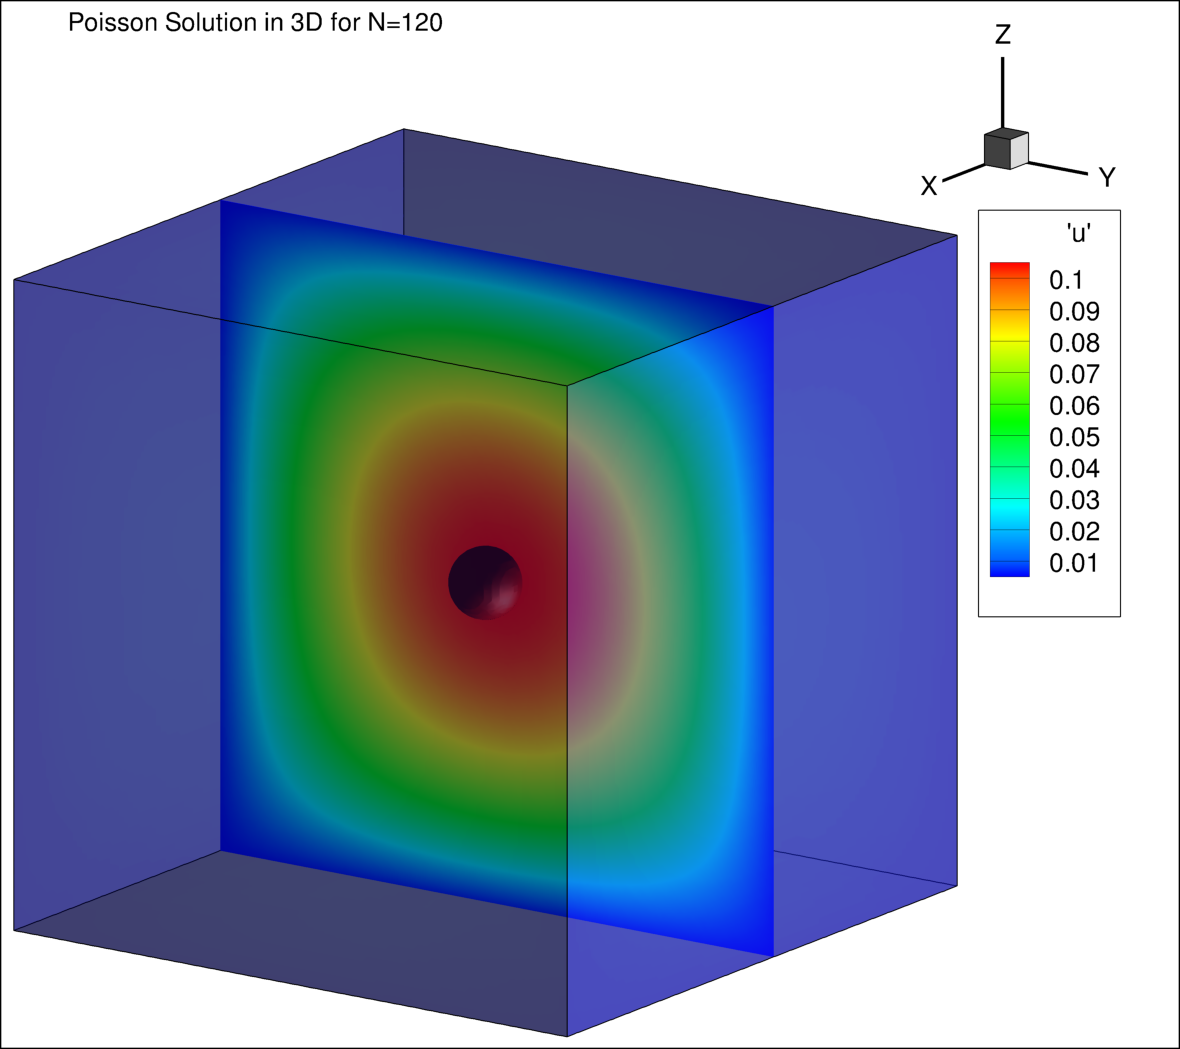
\includegraphics[width=0.7\textheight, trim=0cm 0cm 0 2cm,clip=true]{./figs/3D_Poisson.png}}
\tiny{\caption{\tiny{Solution contours for Poisson problem}}}
\end{figure}
\tiny
\vspace{-15pt}
\[ \text{In 2D:} D=[0,1]^2 , f(x,y)=2(x(1-x)+y(1-y)) \text{ is the source term and }  u(x,y) \text{ is the solution to be computed.} \]
\[\text{Using a } 2^{nd} \text{ order centered finite difference scheme= } -\frac{u_{i+1,j}+u_{i-1,j}+u_{i,j+1}+u_{i,j-1}-4*u_{ij}}{h^2}=f_{ij} \]
\vspace{-5pt}
\[\text{In 3D:} D=[0,1]^3,  f(x,y,z)=3(x(1-x)+y(1-y)+z(1-z)) \text{ is the source term and } u(x,y,z)  \text{ is the solution to be computed.}\]
\[ \text{Using a } 2^{nd} \text{ order centered finite difference scheme:} \]
\[{-\frac{u_{i+1,j,k-1}+u_{i-1,j,k-1}+u_{i,j+1,k-1}+u_{i,j-1,k-1} + u_{i+1,j,k+1}+u_{i-1,j,k+1}+u_{i,j+1,k+1}+u_{i,j-1,k+1}-6 u_{ijk}} {h^2} = f_{ijk}} \]

\end{exampleblock}

\end{minipage}
\end{frame}

%---------------------------------------------------------------------------------------------

%------------------------------------------------------------------------

\begin{frame}
\frametitle{Running already existing LES case on SciNET}
\scriptsize
CFFC code familiarization : LES test case - on parallel clusters - SciNET. Job scheduling and post-processing results (tecplot)
\begin{minipage}[t][1\textheight]{1\textwidth}
\vspace{-10pt}
\begin{exampleblock}{Turbulent premixed $CH_4$ flame, $\phi=0.7$. }
\vspace{-20pt}
\begin{figure}
\label{fig:LES}
\centering
\subfloat[\tiny{Flame temp} \label{fig:flametemp}]{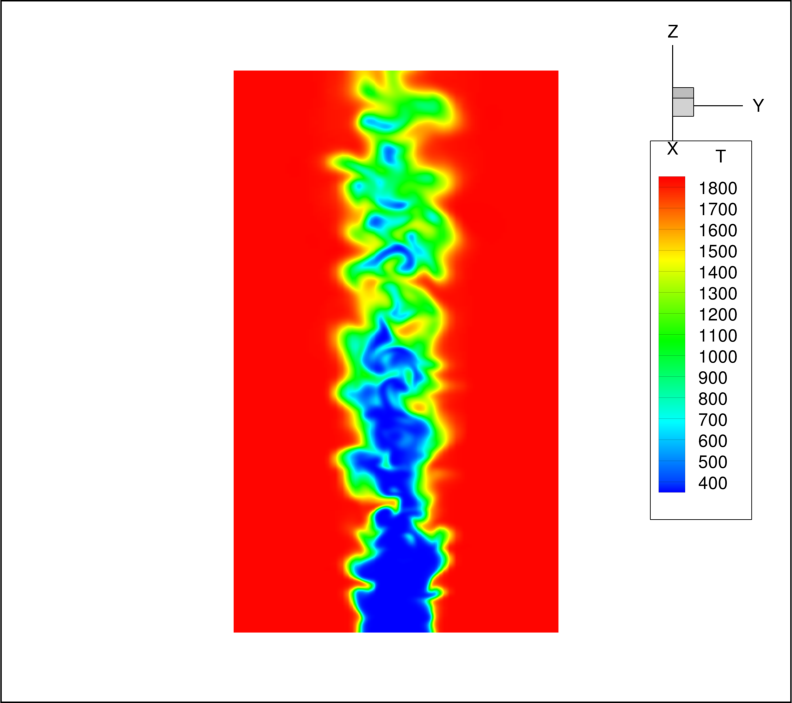
\includegraphics[width=0.2\textheight, trim=7cm 0cm 2cm 0cm,clip=true]{./figs/Flame_temp.png}}
\subfloat[\tiny{FSD, 2.0 ms} \label{fig:fsd2}]{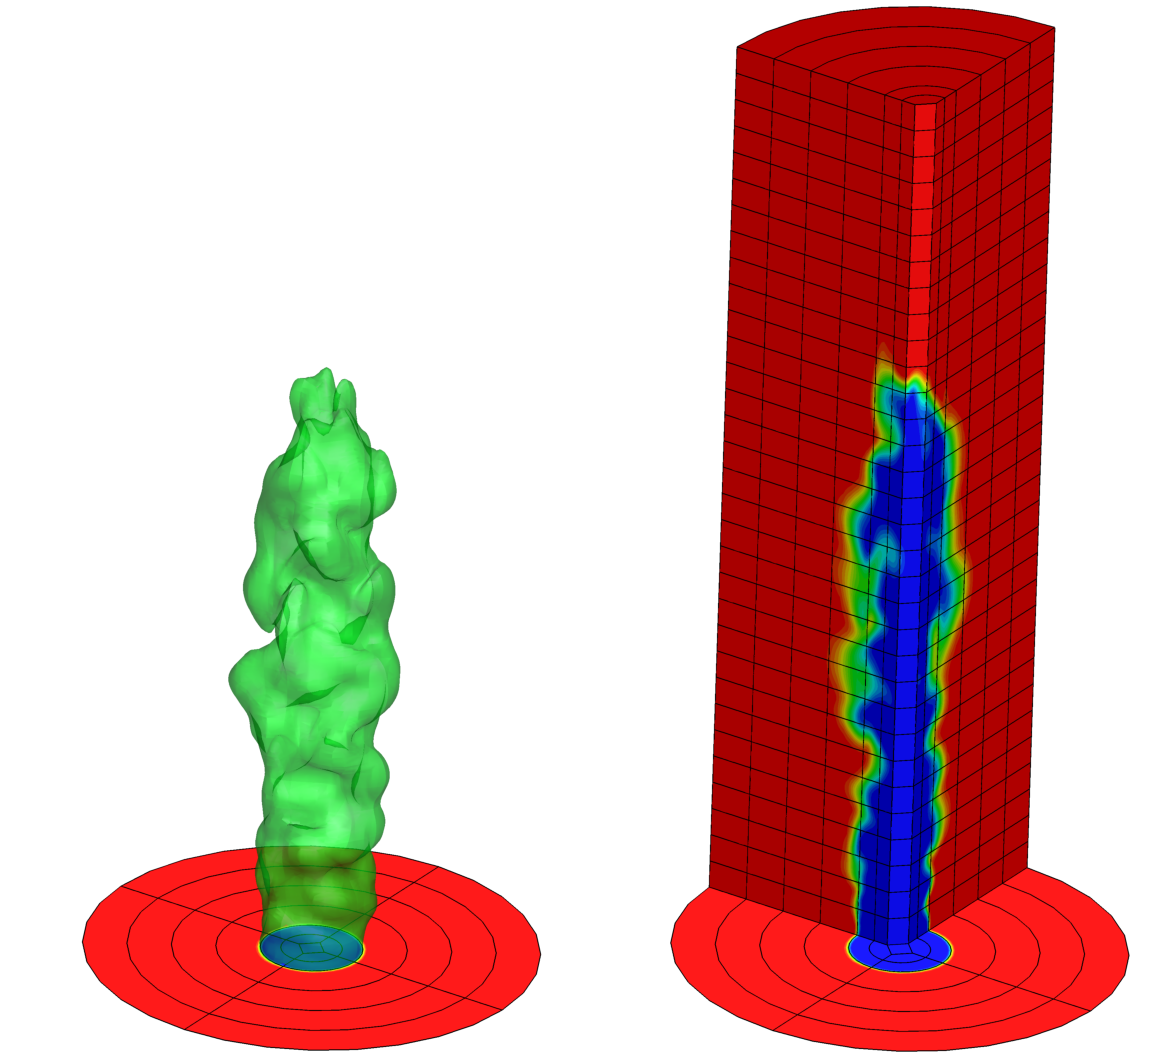
\includegraphics[width=0.3\textheight, trim=0cm 0cm 0 0cm,clip=true]{./figs/fsd2_0ms.png}}
\subfloat[\tiny{FSD, 4.25 ms} \label{fig:fsd4_25}]{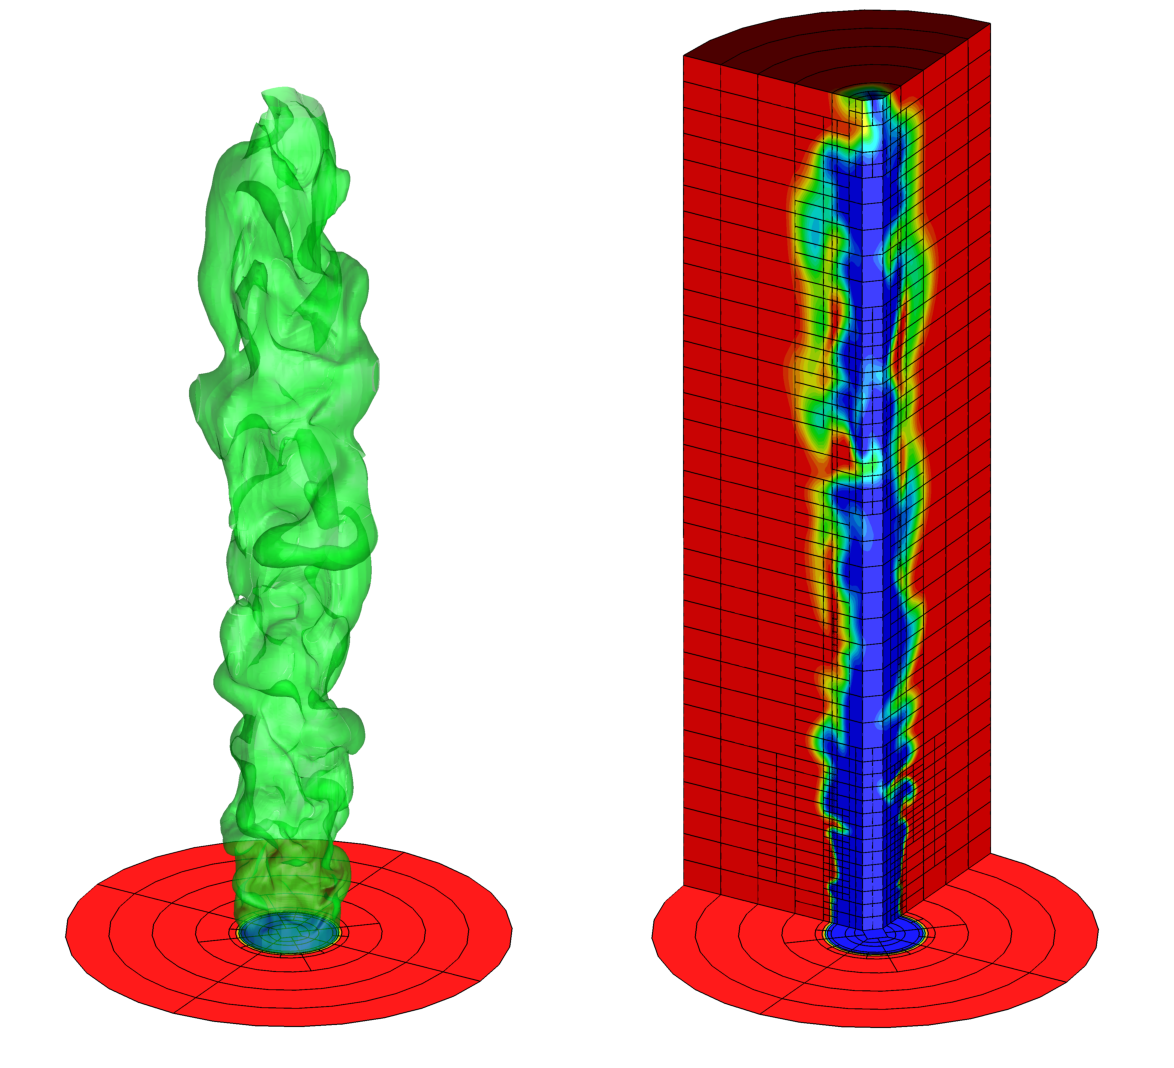
\includegraphics[width=0.3\textheight, trim=0cm 0cm 0 0cm,clip=true]{./figs/fsd4_25ms.png}}
\subfloat[\tiny{FSD, 7.0 ms } \label{fig:fsd7_0}]{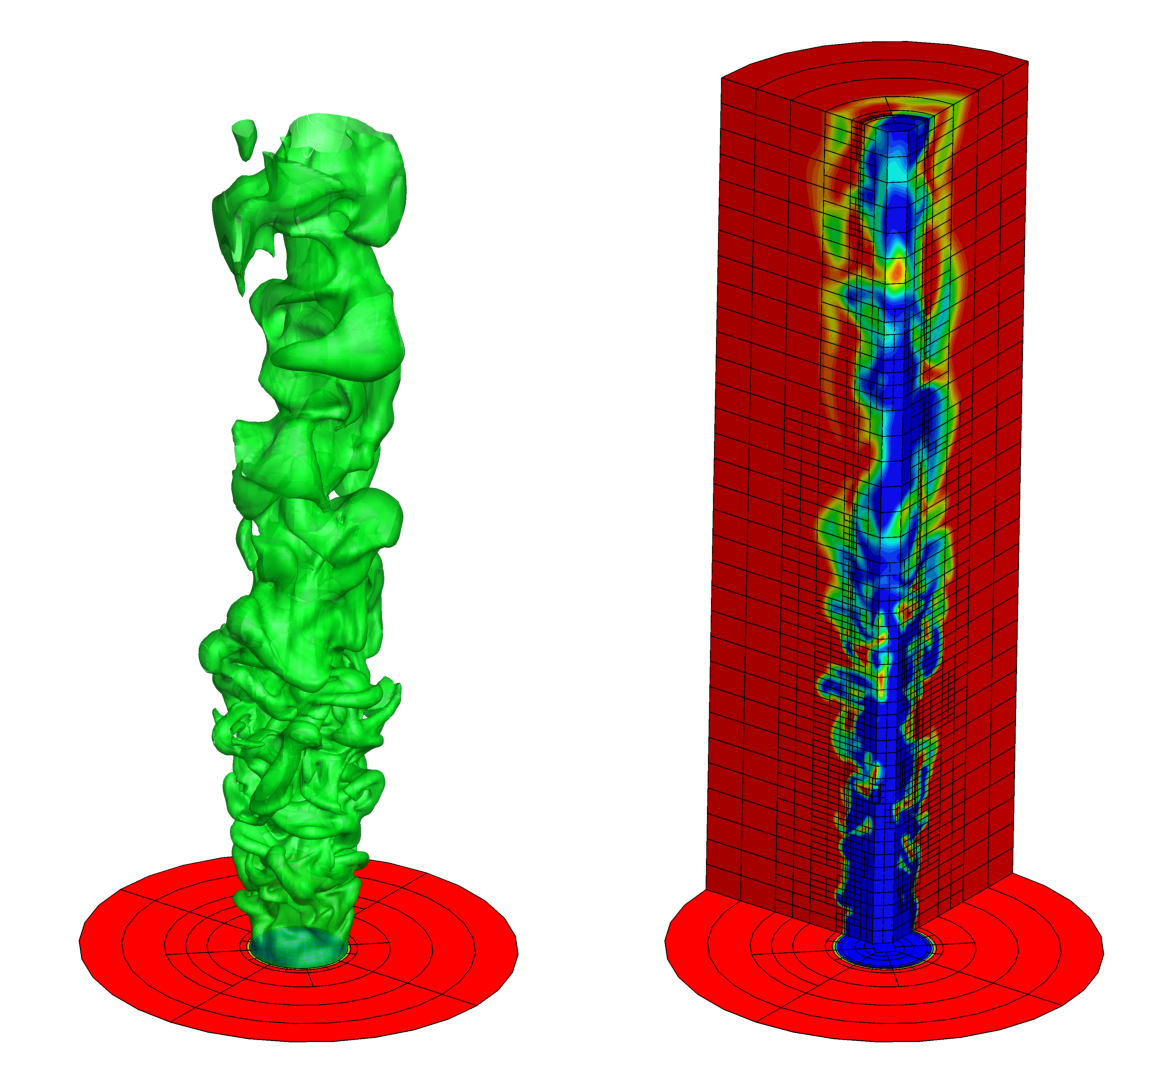
\includegraphics[width=0.3\textheight, trim=0cm 0cm 0 0cm,clip=true]{./figs/fsd7_0ms.png}}
\subfloat[\tiny{time ave $c_{O_{2}}$} \label{fig:tave}]{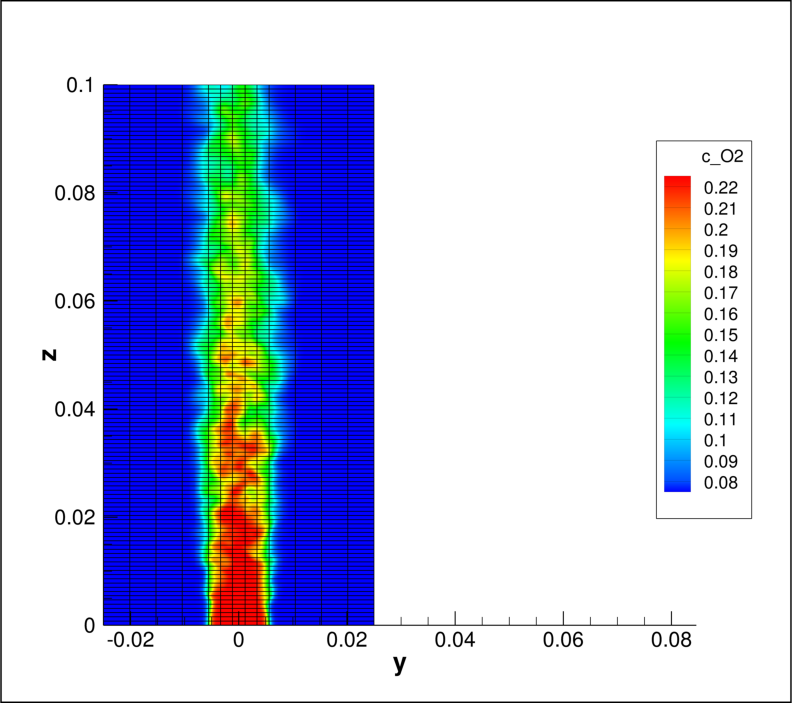
\includegraphics[width=0.25\textheight, trim=4cm 0cm 2cm 0cm,clip=true]{./figs/Time_averaged_c_O2.png}}
%\tiny{\caption{\tiny{Solution contours for Poisson problem}}}
\end{figure}

Computational costs:
\begin{itemize}
\tiny
\item (a) and (e): 800 procs, 3200 (8x8x8) blocks, ~1.64 x$10^6$ cells, no refinement, ~125x$10^3$ CPU hrs 
\item (b) 800 (8x8x8) blocks, ~410,000 cells,  no refinement
\item (c) 5595 (8x8x8) blocks, ~2.8 million cells, 3 levels of mesh refinement
\item (d) 18531 (8x8x8) blocks, ~9.5 million cells, 3 levels of mesh refinement
\end{itemize}

\end{exampleblock}
\end{minipage}


\end{frame}

%------------------------------------------------------------------------


\begin{frame}
\frametitle{Work on the adjoint}
Preliminary work with the discrete adjoint - shockcube problem
\begin{itemize}
\scriptsize
\item give the initial states, l and r
\item how the code was modified - multiblock and multiproc for uniform blocks
\item some results
\item work in progress
\begin{itemize}
\scriptsize
\item boundary conditions
\item compare with other techniques to get dR/dU
\end{itemize}
\end{itemize}

\end{frame}


%==========================================================================
\section[Timeline]{Timeline}

\subsection[Present]{Work done to date}
\begin{frame}%[allowframebreaks]
\frametitle{Timeline: April 2015  - January 2016}
\scriptsize
\begin{itemize}
\item Put a table of what you have done till now
\end{itemize}
\end{frame}


\subsection[Future]{Future work}
\begin{frame}%[allowframebreaks]
\frametitle{Projected milestones}
\scriptsize
\begin{itemize}
\item Put a table of what you will do in the next steps
\end{itemize}
\end{frame}


%==========================================================================
\begin{frame}
\frametitle{Acknowledgements}
\begin{center}
Computations were performed on the GPC supercomputer at the SciNet HPC Consortium. SciNet is funded by: the Canada Foundation for Innovation under the auspices of Compute Canada; the Government of Ontario; Ontario Research Fund - Research Excellence; and the University of Toronto. 
\end{center}
\end{frame}


%==========================================================================
\begin{frame}
\begin{center}
{\huge Thank You For Your Attention!} \\
\vspace*{1.5cm}
{\Large Questions?}
\end{center}
\end{frame}
%==========================================================================

\appendix
\newcounter{finalframe}
\setcounter{finalframe}{\value{framenumber}}

\begin{frame}[allowframebreaks] 
\frametitle{References}
\begin{thebibliography}{1} %Using the bibtex package is recoended but this should allow you do the bibliograghy ad-hoc.
\begin{tiny}
\beamertemplatetextbibitems
\bibitem{MooreLaw}
BCA Research Blog, \newblock {\url{http://blog.bcaresearch.com/wp-content/uploads/2013/10/Chart-III-8-Moores-Law-Over-199-Years-And-Going-Strong.png}}, \newblock Accessed 29-03-2015
\bibitem{Kohler}
K{\"o}hler, M., Boxx, I., Geigle, K. P., and Meier, W., \newblock Simultaneous planar measurements of soot structure and velocity fields in a turbulent lifted jet flame at 3-kHz", \newblock Applied Physics B 103 (2), 271-279, \newblock 2011  
\bibitem{AdelaideISF}
Adelaide international sooting flame (ISF) workshop, \newblock \url{http://www.adelaide.edu.au/cet/isfworkshop/data-sets/turbulent/}, \newblock Accessed 29-03-2015
\bibitem{Pope}
Yang, Y., Pope, S. B., Chen, J. H., \newblock "An LES/PDF study of a turbulent lifted ethylene jet flame in a heated coflow", \newblock 8th US National Combustion Meeting, \newblock 2013
\bibitem{Graetsch}
Gr{\"a}tsch, T., Bathe, K. J., \newblock "A posteriori error estimation techniques in practical finite element analysis", \newblock Journal of Computers and Structures 83, 235–265 ,\newblock 2005 
\bibitem{Bibb}
Bibb, K., Gnoffo, P. A., Park, M. A., Jones, W. T., \newblock "Parallel, Gradient-Based Anisotropic Mesh Adaptation for Re-entry Vehicle Configurations", \newblock AIAA/ASME Joint Thermophysics and Heat Transfer Conference, AIAA Paper 2006–3579, \newblock 2006 
\bibitem{Loken}
Loken, C. et al, \newblock  Journal of Physics: Conf. Ser. 256 012026 , \newblock doi: (10.1088/1742-6596/256/1/012026), \newblock 2010

\end{tiny}
\end{thebibliography}
\end{frame}
%==========================================================================


\begin{frame}
\frametitle{Backup Slide}

\begin{itemize}
\item Important backup slide point.
\end{itemize}

\end{frame}

\setcounter{framenumber}{\value{finalframe}}
\end{document}




%==========================================================================